\section{The harmonic crystal}\label{sec:5.2}

Neutron scattering finds that the vibrations of silicon fill a band from zero up to \SI{64.1}{meV}, organized in six branches over the Brillouin zone. Three of them start at zero energy at the zone center and rise linearly, with slopes between 4.7 and \SI{9.4}{km.s^{-1}}: these are sound waves. Three start at the optical frequency and stay near it. The density of vibrational states piles up in sharp peaks, near \SI{17}{meV}, where the sound waves stop rising, and near \SI{60}{meV}, and a dark-matter particle that deposits energy in single phonons sees these peaks directly in its spectrum. All of this follows from the shape of the energy surface $E^{\mathrm{ad}}(u)$ of \cref{sec:5.1} near its minimum.

\subsection{Force constants and the dynamical matrix}

The displacement of the nucleus $\kappa$ in the cell $\vect{R}$ from its equilibrium site is $\vect{u}_{\vect{R}\kappa}$ (\cref{eq:5.1-X}), and the crystal has $n_{\mathrm{at}}$ nuclei per cell, two for silicon (\cref{sec:3.1}). Expanded about its minimum, the energy surface reads
\begin{equation}
  \begin{gathered}
  E^{\mathrm{ad}}(u) = E^{\mathrm{ad}}(0) + \frac12\sum_{\vect{R}\kappa\alpha}\sum_{\vect{R}'\kappa'\beta}\Phi^{(2),\alpha\beta}_{\kappa\kappa'}(\vect{R},\vect{R}')\,u^\alpha_{\vect{R}\kappa}u^\beta_{\vect{R}'\kappa'} + O(u^3) ,
  \\
  \Phi^{(2),\alpha\beta}_{\kappa\kappa'}(\vect{R},\vect{R}') = \frac{\partial^2E^{\mathrm{ad}}}{\partial u^\alpha_{\vect{R}\kappa}\,\partial u^\beta_{\vect{R}'\kappa'}}\bigg|_{u=0} ,
  \end{gathered}
  \label{eq:5.2-expand}
\end{equation}
with Cartesian indices $\alpha, \beta$. The linear term is absent, since every force vanishes at equilibrium. The coefficients $\Phi^{(2)}$ are the \emph{force constants}: $-\Phi^{(2),\alpha\beta}_{\kappa\kappa'}(\vect{R},\vect{R}')\,u^\beta_{\vect{R}'\kappa'}$ is the force along $\alpha$ on the nucleus $(\vect{R},\kappa)$ when the nucleus $(\vect{R}',\kappa')$ alone is displaced. As second derivatives they are symmetric under interchange of the two nuclei (the pair symmetry), $\Phi^{(2),\alpha\beta}_{\kappa\kappa'}(\vect{R},\vect{R}') = \Phi^{(2),\beta\alpha}_{\kappa'\kappa}(\vect{R}',\vect{R})$, and real. A lattice translation moves every nucleus to an equivalent site and leaves the surface unchanged. As a result the force constants depend on the two cells only through their separation, $\Phi^{(2)}_{\kappa\kappa'}(\vect{R},\vect{R}') = \Phi^{(2)}_{\kappa\kappa'}(\vect{0},\vect{R}'-\vect{R})$. Dropping the terms beyond second order is the \emph{harmonic approximation}. By the counting of \cref{sec:5.1}, the cubic term is smaller than the quadratic one by a factor $\sim\kappa_{\mathrm{BO}}$ at the zero-point amplitude, about \SI{5}{\percent} in silicon (\cref{we:5-kappa}), and we return to it in \cref{sec:5.7}.

The nuclei move in this quadratic potential. We treat their motion classically here. For a Hamiltonian quadratic in the coordinates and momenta, the Heisenberg equations of motion of the displacement operators are the same linear equations as the classical ones, so the normal modes we find are also those of the quantum problem; \cref{sec:5.3} quantizes them. Newton's law for each nucleus is
\begin{equation}
  M_\kappa\,\ddot u^\alpha_{\vect{R}\kappa} = -\frac{\partial E^{\mathrm{ad}}}{\partial u^\alpha_{\vect{R}\kappa}} = -\sum_{\vect{R}'\kappa'\beta}\Phi^{(2),\alpha\beta}_{\kappa\kappa'}(\vect{R},\vect{R}')\,u^\beta_{\vect{R}'\kappa'} ,
  \label{eq:5.2-eom}
\end{equation}
$3n_{\mathrm{at}}N$ coupled linear equations for a crystal of $N$ cells. Two steps reduce them to a small matrix problem: the mass weighting that works for any set of coupled oscillators, and the translation symmetry of the crystal. For a set of coordinates $x_i$ with masses $m_i$ and potential $\tfrac12\sum_{ij}K_{ij}x_ix_j$, the mass-weighted coordinates $y_i = \sqrt{m_i}\,x_i$ obey $\ddot y_i = -\sum_j(K_{ij}/\sqrt{m_im_j})\,y_j$. The matrix on the right is real and symmetric, so it has real eigenvalues $\omega^2$ and orthonormal eigenvectors, and each eigenvector oscillates on its own as $\ee^{-\ii\omega t}$: a normal mode. The crystal is such a system, with one more property. Its matrix is invariant under lattice translations, and a translation-invariant matrix is diagonalized by plane waves in the cell index. We therefore try
\begin{equation}
  u^\alpha_{\vect{R}\kappa}(t) = \frac{1}{\sqrt{M_\kappa}}\,e^\alpha_\kappa\,\ee^{\ii(\vect{Q}\cdot\vect{R} - \omega t)} ,
  \label{eq:5.2-ansatz}
\end{equation}
with a wavevector $\vect{Q}$ and $3n_{\mathrm{at}}$ amplitudes $e^\alpha_\kappa$ to be found. The physical displacement is the real part, or the sum of the solutions at $\vect{Q}$ and $-\vect{Q}$. Inserting \cref{eq:5.2-ansatz} into \cref{eq:5.2-eom}, dividing by $\sqrt{M_\kappa}\,\ee^{\ii(\vect{Q}\cdot\vect{R} - \omega t)}$ and writing $\vect{R}' = \vect{R} + \vect{R}''$, the sum over $\vect{R}''$ no longer depends on $\vect{R}$. What is left is an eigenvalue problem in the $3n_{\mathrm{at}}$ amplitudes,
\begin{equation}
  \sum_{\kappa'\beta}D^{\mathrm{dyn},\alpha\beta}_{\kappa\kappa'}(\vect{Q})\,e^\beta_{\kappa'\nu}(\vect{Q}) = \omega_{\vect{Q}\nu}^2\,e^\alpha_{\kappa\nu}(\vect{Q}) ,
  \qquad
  D^{\mathrm{dyn},\alpha\beta}_{\kappa\kappa'}(\vect{Q}) = \frac{1}{\sqrt{M_\kappa M_{\kappa'}}}\sum_{\vect{R}}\Phi^{(2),\alpha\beta}_{\kappa\kappa'}(\vect{0},\vect{R})\,\ee^{\ii\vect{Q}\cdot\vect{R}} ,
  \label{eq:5.2-Ddyn}
\end{equation}
the \emph{dynamical matrix} $D^{\mathrm{dyn}}(\vect{Q})$, the Fourier transform of the mass-weighted force constants~\cite{born1954dynamical}, \cite[Chaps.~22 and~23]{ashcroft1976solid}, \cite[Eq.~(14)]{giustino2017electron}; it is \cref{eq:A.6-Ddyn}. Its eigenvalues are labeled by the \emph{branch} index $\nu = 1,\dots,3n_{\mathrm{at}}$, and its eigenvectors $\vect{e}_{\kappa\nu}(\vect{Q})$, with one three-vector for each nucleus of the cell, are the \emph{polarization vectors}. The translation symmetry has turned $3n_{\mathrm{at}}N$ equations into $N$ independent problems of size $3n_{\mathrm{at}}$, one for each $\vect{Q}$: six by six for silicon. The phase in \cref{eq:5.2-Ddyn} contains the cell vector $\vect{R}$ and not the position $\vect{R} + \vect{\tau}_\kappa$ of the nucleus. Some codes and texts use the full position; the two choices differ by the phase $\ee^{\ii\vect{Q}\cdot\vect{\tau}_\kappa}$ on each component of $\vect{e}_{\kappa\nu}(\vect{Q})$ and give the same frequencies.

The properties of $D^{\mathrm{dyn}}$ follow from those of $\Phi^{(2)}$. By the pair symmetry of $\Phi^{(2)}$ and translation invariance, $\Phi^{(2),\beta\alpha}_{\kappa'\kappa}(\vect{0},\vect{R}) = \Phi^{(2),\alpha\beta}_{\kappa\kappa'}(\vect{0},-\vect{R})$, and replacing $\vect{R}$ by $-\vect{R}$ in the sum shows that $D^{\mathrm{dyn}}(\vect{Q})$ is Hermitian. Its eigenvalues $\omega_{\vect{Q}\nu}^2$ are therefore real and its eigenvectors orthonormal and complete,
\begin{equation}
  \sum_{\kappa\alpha}e^{\alpha}_{\kappa\nu}(\vect{Q})^*\,e^{\alpha}_{\kappa\nu'}(\vect{Q}) = \delta_{\nu\nu'} , \qquad
  \sum_\nu e^\alpha_{\kappa\nu}(\vect{Q})\,e^\beta_{\kappa'\nu}(\vect{Q})^* = \delta_{\kappa\kappa'}\delta_{\alpha\beta} ,
  \label{eq:5.2-ortho}
\end{equation}
which contains the normalization $\sum_\kappa|\vect{e}_{\kappa\nu}(\vect{Q})|^2 = 1$ of \cref{eq:A.6-e}. At a minimum of $E^{\mathrm{ad}}$ the quadratic form \cref{eq:5.2-expand} is non-negative for every displacement, and so is $D^{\mathrm{dyn}}(\vect{Q})$ for every $\vect{Q}$; every $\omega_{\vect{Q}\nu}^2$ is then non-negative and $\omega_{\vect{Q}\nu}$ real. A computed $\omega_{\vect{Q}\nu}^2 < 0$, usually printed as an imaginary frequency, signals that the structure is not at a minimum, or that the calculation is not converged. Since $\ee^{\ii\vect{G}\cdot\vect{R}} = 1$, $D^{\mathrm{dyn}}(\vect{Q} + \vect{G}) = D^{\mathrm{dyn}}(\vect{Q})$, and $\vect{Q}$ can be taken in the first Brillouin zone: a displacement wave of wavevector $\vect{Q} + \vect{G}$ moves the nuclei exactly as one of wavevector $\vect{Q}$, because the nuclei sit only at the lattice sites. Under Born--von Karman conditions there are $N$ allowed $\vect{Q}$ in the zone (\cref{sec:3.1}), and the crystal has $3n_{\mathrm{at}}N$ modes, one for each degree of freedom. Finally, since the force constants are real, $D^{\mathrm{dyn}}(-\vect{Q}) = D^{\mathrm{dyn}}(\vect{Q})^*$. As a result $\omega_{-\vect{Q}\nu} = \omega_{\vect{Q}\nu}$, and the phases can be chosen so that $\vect{e}_{\kappa\nu}(-\vect{Q}) = \vect{e}_{\kappa\nu}(\vect{Q})^*$, the convention of \cref{eq:A.6-e}.

A quick estimate fixes the scale. The force constant between neighbors is $\Phi^{(2)} \sim \alpha^2m_e/a_0^2 \sim \SI{100}{eV.\angstrom^{-2}}$ by the counting of \cref{sec:5.1}, and the frequencies are $\omega \sim (\Phi^{(2)}/M_\kappa)^{1/2}$. For silicon the zone-center optical mode of \cref{fig:5-scales} has $\Phi_{\mathrm{opt}} = \SI{13.6}{eV.\angstrom^{-2}}$ and $\omega = \SI{63.7}{meV}$ in the same calculation: the estimate is high by a factor of seven in the force constant, and the frequencies are tens of meV.

The force constants are computed, not fitted. Each $\Phi^{(2)}$ is a second derivative of the Kohn--Sham total energy, and density-functional perturbation theory evaluates the whole matrix $D^{\mathrm{dyn}}(\vect{Q})$ at a given $\vect{Q}$ from the linear response of the electrons to a displacement wave. A calculation computes it on a coarse uniform grid of $\vect{Q}$, transforms back to real-space force constants, and evaluates \cref{eq:5.2-Ddyn} at any $\vect{Q}$ from them. The phonons of silicon shown below come from such a calculation.

\begin{workedexample}{The diatomic chain}\label{we:5-chain}
The simplest crystal with both kinds of branch is a line of nuclei of masses $M_1$ and $M_2$, alternating, with period $a_{\mathrm{c}}$ and a spring of stiffness $K$ between neighbors. The nucleus 1 of cell $R$ is tied to the nucleus 2 of the same cell and to the nucleus 2 of the cell $R - a_{\mathrm{c}}$, and the energy is $\tfrac12K\sum_R[(u_{R2} - u_{R1})^2 + (u_{R+a_{\mathrm{c}},1} - u_{R2})^2]$. Differentiating twice, the nonzero force constants from the cell at the origin are $\Phi^{(2)}_{11}(0,0) = \Phi^{(2)}_{22}(0,0) = 2K$, $\Phi^{(2)}_{12}(0,0) = \Phi^{(2)}_{12}(0,-a_{\mathrm{c}}) = -K$ and $\Phi^{(2)}_{21}(0,0) = \Phi^{(2)}_{21}(0,a_{\mathrm{c}}) = -K$. By \cref{eq:5.2-Ddyn},
\begin{equation*}
  D^{\mathrm{dyn}}(Q) = \begin{pmatrix} 2K/M_1 & -K(1 + \ee^{-\ii Qa_{\mathrm{c}}})/\sqrt{M_1M_2} \\ -K(1 + \ee^{\ii Qa_{\mathrm{c}}})/\sqrt{M_1M_2} & 2K/M_2 \end{pmatrix} ,
\end{equation*}
which is Hermitian, as it must be. With $|1 + \ee^{\ii Qa_{\mathrm{c}}}|^2 = 4\cos^2(Qa_{\mathrm{c}}/2)$, the eigenvalues solve $\omega^4 - 2K(M_1^{-1} + M_2^{-1})\,\omega^2 + 4K^2\sin^2(Qa_{\mathrm{c}}/2)/(M_1M_2) = 0$:
\begin{equation*}
  \omega_{Q\pm}^2 = K\Bigl(\frac{1}{M_1} + \frac{1}{M_2}\Bigr) \pm K\Bigl[\Bigl(\frac{1}{M_1} + \frac{1}{M_2}\Bigr)^2 - \frac{4\sin^2(Qa_{\mathrm{c}}/2)}{M_1M_2}\Bigr]^{1/2} .
\end{equation*}
The lower branch vanishes at $Q = 0$. For $Qa_{\mathrm{c}} \ll 1$, expanding the square root to first order in its small term, $\omega_{Q-}^2 = 2K\sin^2(Qa_{\mathrm{c}}/2)/(M_1 + M_2) \simeq KQ^2a_{\mathrm{c}}^2/[2(M_1 + M_2)]$: the frequency is linear in $Q$, a sound wave with speed $c = a_{\mathrm{c}}[K/2(M_1 + M_2)]^{1/2}$, in which the chain moves as a medium of mass $M_1 + M_2$ per length $a_{\mathrm{c}}$. Its eigenvector at $Q = 0$ is $\vect{e} \propto (\sqrt{M_1}, \sqrt{M_2})$, so that by \cref{eq:5.2-ansatz} both nuclei move by the same amount: a rigid translation. This is the \emph{acoustic} branch. The upper branch starts at $\omega_{0+}^2 = 2K/\mu_{\mathrm{red}}$, with $\mu_{\mathrm{red}} = M_1M_2/(M_1 + M_2)$, and its eigenvector at $Q = 0$ is $\vect{e} \propto (\sqrt{M_2}, -\sqrt{M_1})$: the two nuclei move against each other, $u_1/u_2 = -M_2/M_1$, and the center of mass of each cell stays at rest. This is the \emph{optical} branch, so named because, when the two nuclei carry opposite charges, its oscillating dipole couples to light (\cref{sec:5.5}). At the zone boundary, $Q = \pi/a_{\mathrm{c}}$, the off-diagonal elements vanish. Each mode then moves one species only, with $\omega^2 = 2K/M_1$ and $2K/M_2$, and between them lies a gap in which no wave propagates.

For equal masses the gap closes. Then $\omega_{Q\pm} = (2K/M)^{1/2}[1 \pm \cos(Qa_{\mathrm{c}}/2)]^{1/2}$, which is the single branch $\omega = 2(K/M)^{1/2}|\sin(Q'a_{\mathrm{c}}/4)|$ of a chain of identical nuclei with period $a_{\mathrm{c}}/2$, with $Q' = Q$ on the acoustic branch and $Q' = 2\pi/a_{\mathrm{c}} - Q$ on the optical one. The doubled cell has folded the zone in half, and the optical branch is the far half of the acoustic one. Silicon contains exactly this chain. For a wave along $[100]$ with longitudinal polarization, every atomic plane perpendicular to $[100]$ moves rigidly, and the planes, \SI{1.358}{\angstrom} ($a/4$) apart, alternate between the two sublattices of the diamond structure. The two kinds of plane are related by a translation by $a/4$ combined with a rotation by \ang{90} about $[100]$, and the rotation does not affect a longitudinal motion. The planes therefore act as identical masses, and the longitudinal branches along $[100]$ form a folded chain with $a_{\mathrm{c}} = a/2$. Its zone boundary is $Q = 2\pi/a$, the point X. In the folded chain the longitudinal acoustic and optical branches must meet there, whatever the range of the interplanar forces, and in silicon they do, at \SI{12.32}{THz}~\cite{nilsson1972study}.
\end{workedexample}

\subsection{The acoustic sum rule}

The acoustic branch of the chain vanished at $Q = 0$ because a rigid translation costs no energy. This holds for every crystal. Displacing all nuclei by the same vector $\vect{d}$ leaves the energy unchanged at any configuration, $E^{\mathrm{ad}}(u + d) = E^{\mathrm{ad}}(u)$, where $u + d$ means $\vect{u}_{\vect{R}\kappa} + \vect{d}$ for every nucleus. Differentiating with respect to $u^\alpha_{\vect{R}\kappa}$ and to $d^\beta$, and setting $u = d = 0$, yields $\sum_{\vect{R}'\kappa'}\partial^2E^{\mathrm{ad}}/\partial u^\alpha_{\vect{R}\kappa}\partial u^\beta_{\vect{R}'\kappa'} = 0$, that is
\begin{equation}
  \sum_{\vect{R}\kappa'}\Phi^{(2),\alpha\beta}_{\kappa\kappa'}(\vect{0},\vect{R}) = 0 \qquad \text{for every } \kappa, \alpha, \beta .
  \label{eq:5.2-asr}
\end{equation}
This is the \emph{acoustic sum rule}: the force on a nucleus when all others, and the nucleus itself, are moved together vanishes. Its consequence for the dynamical matrix follows at once. At $\vect{Q} = 0$, the vector $e^\beta_{\kappa'} = (M_{\kappa'}/M_{\mathrm{cell}})^{1/2}\hat e^\beta$, with $M_{\mathrm{cell}} = \sum_\kappa M_\kappa$ and any unit vector $\hat{\vect{e}}$, gives $\sum_{\kappa'\beta}D^{\mathrm{dyn},\alpha\beta}_{\kappa\kappa'}(\vect{0})\,e^\beta_{\kappa'} = (M_\kappa M_{\mathrm{cell}})^{-1/2}\sum_\beta\bigl[\sum_{\vect{R}\kappa'}\Phi^{(2),\alpha\beta}_{\kappa\kappa'}(\vect{0},\vect{R})\bigr]\hat e^\beta = 0$. Three independent choices of $\hat{\vect{e}}$ give three modes of zero frequency at the zone center, the \emph{acoustic} branches, in which all nuclei move together. These are the polarization vectors of \cref{app:A.6}, $\vect{e}_{\kappa\nu} = (M_\kappa/M_{\mathrm{cell}})^{1/2}\hat{\vect{e}}_\nu$. The other $3n_{\mathrm{at}} - 3$ branches, three in silicon, are the \emph{optical} branches, finite at $\vect{Q} = 0$. In them the nuclei of a cell move against each other with their center of mass at rest: orthogonality to the three acoustic vectors in \cref{eq:5.2-ortho} is $\sum_\kappa\sqrt{M_\kappa}\,\vect{e}_{\kappa\nu}(\vect{0}) = 0$, and the displacement $\vect{e}_{\kappa\nu}/\sqrt{M_\kappa}$ of \cref{eq:5.2-ansatz} then has $\sum_\kappa M_\kappa\,\vect{u}_\kappa = 0$. In field-theory language the acoustic phonons are the Goldstone modes of the translation symmetry that the crystal breaks~\cite[p.~69]{lin2019tasi}. A uniform translation is a different ground state at the same energy, and a translation that varies slowly in space costs an energy that vanishes as its wavelength grows.

A computed set of force constants violates \cref{eq:5.2-asr} slightly, chiefly because the exchange--correlation potential is evaluated on a real-space grid that is not invariant under arbitrary translations. The acoustic frequencies at $\mathrm{\Gamma}$ then come out small but nonzero, \SI{0.16}{THz} in the calculation of \cref{fig:5-si}, and codes restore the rule by correcting the on-site constants.

\subsection{Sound speeds}

Near $\vect{Q} = 0$ the acoustic frequencies rise from zero, and we want the rate at which they do. Expanding the exponential in \cref{eq:5.2-Ddyn} in powers of $\vect{Q}$,
\begin{equation}
  \begin{gathered}
  D^{\mathrm{dyn}}(\vect{Q}) = D_0 + D_1(\vect{Q}) + D_2(\vect{Q}) + O(Q^3) , \\
  D^{\alpha\beta}_{n,\kappa\kappa'}(\vect{Q}) = \frac{1}{\sqrt{M_\kappa M_{\kappa'}}}\sum_{\vect{R}}\Phi^{(2),\alpha\beta}_{\kappa\kappa'}(\vect{0},\vect{R})\,\frac{(\ii\vect{Q}\cdot\vect{R})^n}{n!} ,
  \end{gathered}
  \label{eq:5.2-Dexp}
\end{equation}
and treating $D_1$ and $D_2$ as perturbations of $D_0 = D^{\mathrm{dyn}}(\vect{0})$, whose acoustic eigenvalue is triply degenerate at zero, leads to $\omega^2$ as an expansion in $Q$. The acoustic frequencies are the eigenvalues of a $3\times3$ matrix in the space of the three acoustic vectors $\vect{a}_{\hat{\vect{e}}}$, with components $(M_\kappa/M_{\mathrm{cell}})^{1/2}\hat{\vect{e}}$.

The first-order term would make $\omega^2$ linear in $Q$, and $\omega \propto Q^{1/2}$, which no crystal shows. Rotational invariance makes it vanish. Its matrix elements are
\begin{equation*}
  \vect{a}_{\hat{\vect{e}}}^\dagger D_1\,\vect{a}_{\hat{\vect{e}}'} = \frac{\ii Q_\gamma}{M_{\mathrm{cell}}}\,\hat e^\alpha\hat e'^\beta\,T^{\alpha\beta\gamma} , \qquad
  T^{\alpha\beta\gamma} = \sum_{\kappa\kappa'\vect{R}}\Phi^{(2),\alpha\beta}_{\kappa\kappa'}(\vect{0},\vect{R})\,R^\gamma ,
\end{equation*}
with summation over repeated Cartesian indices. Two properties of $T$ force it to zero. The first follows from the pair symmetry of $\Phi^{(2)}$. Writing $\Phi^{(2),\beta\alpha}_{\kappa\kappa'}(\vect{0},\vect{R}) = \Phi^{(2),\alpha\beta}_{\kappa'\kappa}(\vect{0},-\vect{R})$ and relabeling $\kappa \leftrightarrow \kappa'$ and $\vect{R} \to -\vect{R}$ in the sum shows $T^{\beta\alpha\gamma} = -T^{\alpha\beta\gamma}$. The second follows from rotations. A rigid infinitesimal rotation by the angle vector $\vect{\theta}$ moves every nucleus, at whatever position $\vect{X}_I$ it has, by $\vect{\theta}\times\vect{X}_I$ and leaves the energy unchanged. (For a crystal under Born--von Karman conditions a rotation is not a symmetry, but the force constants are those of a large free crystal, for which it is.) Hence $\sum_I\nabla_IE^{\mathrm{ad}}\cdot(\vect{\theta}\times\vect{X}_I) = 0$ at every configuration: the total torque vanishes. Differentiating this identity with respect to the displacement of one nucleus and evaluating at equilibrium, where the forces vanish, leaves $\sum_I\Phi^{(2)}_{JI}\,(\vect{\theta}\times\vect{X}_I) = 0$ for every $J$ and every $\vect{\theta}$. In components, $\sum_{\vect{R}\kappa'}\Phi^{(2),\alpha\beta}_{\kappa\kappa'}(\vect{0},\vect{R})\,X^\gamma_{\vect{R}\kappa'}$ is symmetric in $\beta\gamma$, with $\vect{X}_{\vect{R}\kappa'} = \vect{R} + \vect{\tau}_{\kappa'}$. Summed over $\kappa$, it is $T^{\alpha\beta\gamma}$ plus a term $\sum_{\kappa\kappa'}[\sum_{\vect{R}}\Phi^{(2)}_{\kappa\kappa'}(\vect{0},\vect{R})]\tau^\gamma_{\kappa'}$, which vanishes because the sum rule \cref{eq:5.2-asr} also holds with the roles of $\kappa$ and $\kappa'$ exchanged (by the same pair symmetry). So $T^{\alpha\beta\gamma}$ is symmetric in $\beta\gamma$ and antisymmetric in $\alpha\beta$, and a tensor with both properties is zero. Alternating the two properties six times returns to the start with a minus sign~\cite[Chap.~V]{born1954dynamical}:
\begin{equation*}
  T^{\alpha\beta\gamma} = -T^{\beta\alpha\gamma} = -T^{\beta\gamma\alpha} = T^{\gamma\beta\alpha} = T^{\gamma\alpha\beta} = -T^{\alpha\gamma\beta} = -T^{\alpha\beta\gamma} = 0 .
\end{equation*}

At second order two terms contribute. One is the expectation value of $D_2$ in the acoustic space. The other is $D_1$ taken twice, through the optical modes: $D_1$ does connect an acoustic vector to an optical one at $\vect{Q} = 0$, with frequency $\omega_{\mathrm{o}}$, and second-order perturbation theory adds $-|\vect{o}^\dagger D_1\vect{a}_{\hat{\vect{e}}}|^2/\omega_{\mathrm{o}}^2$. Both are quadratic in $\vect{Q}$, so
\begin{equation}
  \omega_{\vect{Q}\nu}^2 = \Lambda^{\mathrm{ac}}_\nu(\hat{\vect{Q}})\,Q^2 + O(Q^3), \qquad
  \omega_{\vect{Q}\nu} = c_\nu(\hat{\vect{Q}})\,Q , \qquad c_\nu(\hat{\vect{Q}}) = \Lambda^{\mathrm{ac}}_\nu(\hat{\vect{Q}})^{1/2} ,
  \label{eq:5.2-sound}
\end{equation}
where $\Lambda^{\mathrm{ac}}_\nu(\hat{\vect{Q}})$ are the three eigenvalues of the $3\times3$ matrix
\begin{equation*}
  \Lambda^{\mathrm{ac},\alpha\beta}(\hat{\vect{Q}})\,Q^2 = -\frac{1}{2M_{\mathrm{cell}}}\sum_{\kappa\kappa'\vect{R}}\Phi^{(2),\alpha\beta}_{\kappa\kappa'}(\vect{0},\vect{R})\,(\vect{Q}\cdot\vect{R})^2
  - \sum_{\mathrm{o}}\frac{(\vect{a}_\alpha^\dagger D_1\vect{o})(\vect{o}^\dagger D_1\vect{a}_\beta)}{\omega_{\mathrm{o}}^2} ,
\end{equation*}
with $\vect{a}_\alpha$ the acoustic vector polarized along the axis $\alpha$ and the sum over the optical modes at $\vect{Q} = 0$. The frequency of an acoustic mode is linear in $Q$, with a sound speed $c_\nu(\hat{\vect{Q}})$ that depends on the direction of propagation and on the branch, and the polarizations $\hat{\vect{e}}_\nu(\hat{\vect{Q}})$ are the eigenvectors of $\Lambda^{\mathrm{ac}}$. The first term is the stiffness of the crystal when every nucleus follows the long wave rigidly, the sum of the springs weighted by the squared lengths over which they are stretched. The second lowers it. In a crystal with more than one nucleus per cell, a strain pushes the sublattices against each other, and the optical coordinate relaxes in the long wave; this internal relaxation, which in the diamond structure reduces the shear stiffness, is what the second term describes~\cite[Chap.~V]{born1954dynamical}. In silicon the first-order coupling $D_1$ from acoustic to optical vectors vanishes for the longitudinal wave along $[100]$, in which the planes of \cref{we:5-chain} move as identical masses and the two sublattices are not pushed against each other, but not for shear waves.

Since $\Lambda^{\mathrm{ac}}$ describes a long wave, it is a property of the crystal as an elastic continuum. \Cref{app:C.18} derives the equation of motion of such a continuum, the Christoffel equation, with the elastic constants $C_{ijkl}$ and the mass density $\rho_T$, and \cref{eq:5.2-sound} is the same equation: $\rho_T\Lambda^{\mathrm{ac}}$, with $\rho_T = M_{\mathrm{cell}}/\Omega$, is the Christoffel matrix of the relaxed elastic constants. For a cubic crystal along $[100]$ this reads $\rho_Tc_{\mathrm{LA}}^2 = C_{11}$ and $\rho_Tc_{\mathrm{TA}}^2 = C_{44}$ for the two degenerate transverse branches. The sound speeds of the dark-matter kinematics of \cref{sec:1.3} are these slopes, and the acoustic edge $m^{\mathrm{ac}}_{\mathrm{min}}$ of \cref{sec:9.2} uses them. The longitudinal speed is the largest, since compressing a medium costs more than shearing it. The scale is a vibrational frequency $(\Phi^{(2)}/M_\kappa)^{1/2}$ times a distance of the order of the spacing between atomic planes: for silicon, the optical frequency times $a/4$ is \SI{13}{km.s^{-1}}, against measured speeds of 4.7 to \SI{9.4}{km.s^{-1}}. Note that $c/v_{\mathrm{max}} \sim 10^{-2}$: sound is two orders of magnitude slower than the fastest dark matter, which is why an acoustic phonon takes only a small fraction of the kinetic energy (\cref{sec:1.3}).

\subsection{The phonons of silicon}

\Cref{fig:5-si}(a) shows the six branches of silicon along the three lines of the zone on which they were measured: from $\mathrm{\Gamma}$ to X along $[100]$, from X to $\mathrm{\Gamma}$ along $[110]$ through K, and from $\mathrm{\Gamma}$ to L along $[111]$. On these lines the symmetry of the crystal makes every polarization either parallel or perpendicular to $\vect{Q}$, and the branches are named accordingly: longitudinal and transverse acoustic (LA, TA), longitudinal and transverse optical (LO, TO). In a general direction the polarizations mix, and the names refer to the branch that is mostly longitudinal or mostly transverse. Along $[100]$ and $[111]$ the two transverse branches of each kind are degenerate by the symmetry of these axes; along $[110]$ they split.

The measured frequencies at the high-symmetry points come from inelastic neutron scattering at room temperature~\cite{dolling1963inelastic,nilsson1972study}. At $\mathrm{\Gamma}$ the three optical modes are degenerate, at \SI{15.5}{THz}, or \SI{64.1}{meV}. In a polar crystal the longitudinal one would be pushed up by the electric field it creates, the LO--TO splitting of \cref{sec:5.5}; silicon has no Born charges and no splitting. At X the longitudinal acoustic and optical branches meet, at \SI{12.32}{THz} (\SI{50.95}{meV}), as the folded chain of \cref{we:5-chain} requires. Near the zone boundary the transverse acoustic branches bend over and become almost flat, at \SI{4.49}{THz} (\SI{18.6}{meV}) at X and \SI{3.43}{THz} (\SI{14.2}{meV}) at L. The reason is the covalent bond. Stretching a bond is stiff, while changing the angle between two bonds is soft, and a short-wavelength transverse wave mostly bends bonds. Finally, the optical branches are narrow. From \SI{15.5}{THz} at $\mathrm{\Gamma}$ they fall only to between 12.3 and \SI{14.7}{THz} at the zone boundary. The reason is that the motion of the two atoms of a cell against each other is controlled by the stiff bond between them and depends only weakly on what the neighboring cells do.

The lines in \cref{fig:5-si}(a) are a density-functional calculation with the PBE functional at the measured lattice constant, from force constants computed by density-functional perturbation theory (DFPT) on a $6^3$ grid of wavevectors. They follow the measurements closely. Of the eight measured frequencies at $\mathrm{\Gamma}$, X and L, six agree to within \SI{2}{\percent}, and the mean absolute difference over all eight is \SI{2.6}{\percent}. The zone-center optical mode comes out at \SI{15.40}{THz} (\SI{63.7}{meV}), \SI{0.6}{\percent} below the measured \SI{64.1}{meV} and the same as the frozen-phonon value of \cref{fig:5-scales}. The exceptions are the flat transverse acoustic modes, \SI{8}{\percent} soft: \num{4.13} against \SI{4.49}{THz} at X and \num{3.17} against \SI{3.43}{THz} at L. PBE generally puts the phonons of silicon and germanium below the measured ones, a consequence of its underbinding~\cite[Sect.~V]{haxhijaj2026lattice}; in this calculation the deficit is largest on the branches set by bond bending, the weakest force constant of the crystal. The calculation describes a static lattice, while the measurement was made at room temperature, where the frequencies are lower by thermal expansion and by anharmonic shifts; these effects, and the widths $\gamma_{\vect{Q}\nu}$ that the harmonic crystal lacks entirely, are the subject of \cref{sec:5.7}. A frequency also moves with the lattice constant at which it is computed, by an amount set by its Grüneisen parameter $\gamma^{\mathrm{G}}_{\vect{Q}\nu} = -\partial\ln\omega_{\vect{Q}\nu}/\partial\ln\Omega$. For most modes of silicon $\gamma^{\mathrm{G}}_{\vect{Q}\nu} > 0$, and the PBE lattice constant, \SI{0.85}{\percent} too large, would soften them; the flat transverse acoustic modes have $\gamma^{\mathrm{G}}_{\vect{Q}\nu} < 0$ and would stiffen.

\begin{figure}[tbp]
  \centering
  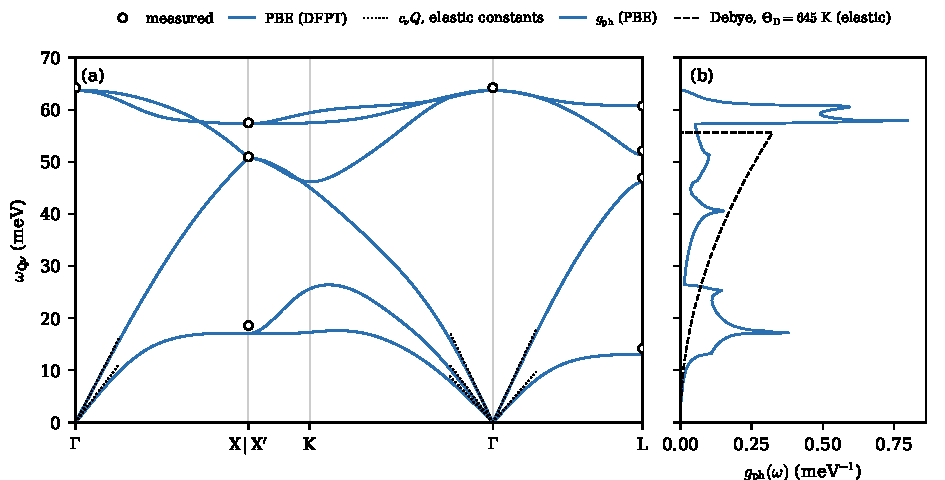
\includegraphics[width=\linewidth]{figures/ch05/fig5_2.pdf}
  \caption{Phonons of silicon. (a) Dispersion along $[100]$ from $\mathrm{\Gamma}$ to X, along $[110]$ from X$'$ $= (1,1,0)2\pi/a$, which is equivalent to X, through K to $\mathrm{\Gamma}$, and along $[111]$ from $\mathrm{\Gamma}$ to L. Lines: density-functional perturbation theory with the PBE functional, an SG15 norm-conserving pseudopotential, a \SI{60}{Ry} cutoff, a $12^3$ grid of crystal momenta, the measured lattice constant $a = \SI{5.431}{\angstrom}$ and the natural mass of silicon; force constants from a $6^3$ grid of wavevectors, with the acoustic sum rule imposed, interpolated to the path. Circles: frequencies measured by inelastic neutron scattering at room temperature at $\mathrm{\Gamma}$, X and L~\cite{dolling1963inelastic,nilsson1972study}, as tabulated in Ref.~\cite[Table~I]{savrasov1996linear}. Dotted: $\omega = c_\nu Q$ with the sound speeds of the measured elastic constants (\cref{we:5-debye}), drawn up to $Q = 0.25\,(2\pi/a)$. (b) Phonon density of states per two-atom cell, normalized to six modes, from the same force constants on a $48^3$ grid (tetrahedron integration), and the Debye model \cref{eq:5.2-gD} with $\bar c$ from the measured elastic constants, $\omega_{\mathrm{D}} = \SI{55.6}{meV}$, in the convention of one wavevector per atom. One THz corresponds to \SI{4.136}{meV}.}
  \label{fig:5-si}
\end{figure}

\subsection{The density of states}

For any quantity that sums over all phonons, such as a rate summed over final states or a thermal average, what matters is how many modes there are at each frequency. The phonon density of states per cell is
\begin{equation}
  g_{\mathrm{ph}}(\omega) = \frac1N\sum_{\vect{Q}\nu}\delta(\omega - \omega_{\vect{Q}\nu}) = \frac{\Omega}{(2\pi)^3}\sum_\nu\int_{\mathrm{BZ}}\dd^3Q\;\delta(\omega - \omega_{\vect{Q}\nu}) ,
  \qquad \int_0^\infty\dd\omega\,g_{\mathrm{ph}}(\omega) = 3n_{\mathrm{at}} ,
  \label{eq:5.2-dos}
\end{equation}
where the sum over the $N$ wavevectors of the zone became an integral with the density $\Vol/(2\pi)^3$ of \cref{sec:3.1}, $\Vol = N\Omega$. Its integral counts the $3n_{\mathrm{at}}$ modes per cell, six for silicon. A density of states per atom, normalized to three, is $g_{\mathrm{ph}}/n_{\mathrm{at}}$. In silicon, \cref{fig:5-si}(b), $g_{\mathrm{ph}}$ has a sharp peak at \SI{17}{meV} from the flat transverse acoustic branches near the zone boundary. Above it lies a structured region between 25 and \SI{52}{meV} from the longitudinal acoustic branch and the lower optical branches. The tallest peaks, at 58 and \SI{61}{meV}, come from the flat transverse optical branches. The peaks are where the branches are flat. Near a frequency at which $\nabla_{\vect{Q}}\omega_{\vect{Q}\nu}$ vanishes, many wavevectors share nearly the same frequency, and in three dimensions the density of states has a kink with an infinite slope there, a Van Hove singularity~\cite[Chap.~23]{ashcroft1976solid}. The large peak of the transverse acoustic branches is what makes silicon's low-energy phonons so numerous: a dark-matter particle that can deposit \SI{20}{meV} in single phonons finds a fifth of all modes of the crystal, \SI{22}{\percent} in the calculation, below that energy.

At low frequency only the acoustic branches contribute, with $\omega_{\vect{Q}\nu} = c_\nu(\hat{\vect{Q}})Q$. Writing $\dd^3Q = Q^2\dd Q\,\dd\hat{\vect{Q}}$ and integrating over $Q$ with $\int Q^2\dd Q\,\delta(\omega - c_\nu Q) = \omega^2/c_\nu^3$,
\begin{equation}
  g_{\mathrm{ph}}(\omega) \simeq \frac{\Omega\,\omega^2}{2\pi^2}\sum_\nu\bigl\langle c_\nu^{-3}\bigr\rangle , \qquad
  \bigl\langle c_\nu^{-3}\bigr\rangle = \int\frac{\dd\hat{\vect{Q}}}{4\pi}\,c_\nu(\hat{\vect{Q}})^{-3} ,
  \label{eq:5.2-dosac}
\end{equation}
an $\omega^2$ law with a coefficient fixed by the sound speeds alone, averaged over directions. It holds as long as the dispersion is linear, which in silicon means up to about \SI{7}{meV}, where the computed $g_{\mathrm{ph}}$ exceeds the $\omega^2$ law by \SI{10}{\percent}.

\subsection{The Debye model}

Debye's model extends \cref{eq:5.2-dosac} to the whole spectrum. It replaces the $3n_{\mathrm{at}}$ branches by three, all with the linear dispersion $\omega = \bar cQ$ of a single averaged speed $\bar c$. It also replaces the zone by a sphere of radius $Q_{\mathrm{D}}$ that holds one wavevector per atom, $n_{\mathrm{at}}N$ in all, so that the three branches carry all $3n_{\mathrm{at}}N$ degrees of freedom~\cite[Chap.~23]{ashcroft1976solid}. Counting with the density $\Vol/(2\pi)^3$, $(4\pi Q_{\mathrm{D}}^3/3)\,N\Omega/(2\pi)^3 = n_{\mathrm{at}}N$, so that
\begin{equation}
  Q_{\mathrm{D}} = \Bigl(\frac{6\pi^2n_{\mathrm{at}}}{\Omega}\Bigr)^{1/3} , \qquad
  \omega_{\mathrm{D}} = \bar c\,Q_{\mathrm{D}} , \qquad
  \Theta_{\mathrm{D}} = \omega_{\mathrm{D}} ,
  \label{eq:5.2-debye}
\end{equation}
with the Debye frequency $\omega_{\mathrm{D}}$ and the Debye temperature $\Theta_{\mathrm{D}}$, which in natural units are the same number. The density of states of the model follows from \cref{eq:5.2-dosac} with $c_\nu = \bar c$, cut off at $\omega_{\mathrm{D}}$:
\begin{equation}
  g_{\mathrm{D}}(\omega) = \frac{3\Omega\,\omega^2}{2\pi^2\bar c^3}\,\Theta(\omega_{\mathrm{D}} - \omega) = \frac{9n_{\mathrm{at}}\,\omega^2}{\omega_{\mathrm{D}}^3}\,\Theta(\omega_{\mathrm{D}} - \omega) ,
  \label{eq:5.2-gD}
\end{equation}
where the second form uses \cref{eq:5.2-debye}; its integral is $3n_{\mathrm{at}}$, as it must be. Matching the low-frequency limit \cref{eq:5.2-dosac} exactly fixes the speed,
\begin{equation}
  \frac{3}{\bar c^3} = \sum_\nu\bigl\langle c_\nu^{-3}\bigr\rangle .
  \label{eq:5.2-cbar}
\end{equation}
This is the definition we use. It makes the model exact wherever only long acoustic waves matter, as in the heat capacity at low temperature, which then follows Debye's $T^3$ law with this $\Theta_{\mathrm{D}}$, and in a dark-matter rate dominated by the lowest phonon energies. Since $c^{-3}$ is averaged, the slowest branches dominate $\bar c$. Note that the literature also uses a second convention. Some texts, particularly on phonon transport, put only the $N$ acoustic wavevectors in the sphere, one per cell, which lowers $Q_{\mathrm{D}}$ and $\Theta_{\mathrm{D}}$ by the factor $n_{\mathrm{at}}^{1/3}$, $2^{1/3} = 1.26$ for silicon, and treats the optical branches separately.

Above a few meV, however, the model is crude. It puts all modes below $\omega_{\mathrm{D}}$, and in silicon it misses both the peak of the flat transverse branches and the optical band at the top. Its strength is that one number fixes the low-energy spectrum, and any quantity that is an integral over $g_{\mathrm{ph}}$ weighted toward low frequencies, such as the mean-square displacement at room temperature (\cref{sec:5.3}) or the Debye--Waller exponent (\cref{sec:5.6}), comes out within tens of percent. \Cref{we:5-debye} carries this through for silicon.

\begin{workedexample}{Silicon sound speeds and Debye temperature}\label{we:5-debye}
The elastic constants of silicon at room temperature are $C_{11} = \SI{165.6}{GPa}$, $C_{12} = \SI{63.9}{GPa}$ and $C_{44} = \SI{79.5}{GPa}$, and its density is $\rho_T = \SI{2.33}{g.cm^{-3}}$~\cite[Table~I]{martinez2019measurements}. Along $[100]$, $\rho_Tc_{\mathrm{LA}}^2 = C_{11}$ and $\rho_Tc_{\mathrm{TA}}^2 = C_{44}$, so
\begin{gather*}
  c_{\mathrm{LA}} = \Bigl(\frac{\SI{165.6e9}{Pa}}{\SI{2330}{kg.m^{-3}}}\Bigr)^{1/2} = \SI{8.43}{km.s^{-1}} , \\
  c_{\mathrm{TA}} = \Bigl(\frac{\SI{79.5e9}{Pa}}{\SI{2330}{kg.m^{-3}}}\Bigr)^{1/2} = \SI{5.84}{km.s^{-1}}\ (\text{twice}) .
\end{gather*}
In other directions the speeds are the eigenvalues of the Christoffel matrix (\cref{app:C.18}): along $[110]$, 9.13 for LA and 5.84 and \SI{4.67}{km.s^{-1}} for the two TA branches; along $[111]$, 9.35 for LA and \SI{5.09}{km.s^{-1}} for both TA branches. The longitudinal speed varies by \SI{11}{\percent} with direction and the transverse ones by \SI{25}{\percent}. These are the slopes of the acoustic branches at $\mathrm{\Gamma}$ in \cref{fig:5-si}(a). The PBE calculation of that figure, interpolated from its $6^3$ grid to small $Q$, has 8.34 and \SI{5.44}{km.s^{-1}} along $[100]$, \SI{1}{\percent} and \SI{7}{\percent} below; its transverse branches are soft at small $Q$ as they are at X and L.

The Debye speed \cref{eq:5.2-cbar} needs the average of $c_\nu^{-3}$ over all directions, which we evaluate numerically by diagonalizing the Christoffel matrix on a fine grid of directions. Ordering the three branches by speed in each direction, the averages $\langle c_\nu^{-3}\rangle^{-1/3}$ are 9.00, 5.66 and \SI{5.04}{km.s^{-1}}, and
\begin{equation*}
  \bar c = \Bigl[\frac{3}{\sum_\nu\langle c_\nu^{-3}\rangle}\Bigr]^{1/3} = \SI{5.89}{km.s^{-1}} ,
\end{equation*}
closer to the transverse speeds than to the longitudinal one: the longitudinal branch contributes only \SI{9}{\percent} of $\sum_\nu\langle c_\nu^{-3}\rangle$. With $n_{\mathrm{at}}/\Omega = 8/a^3 = \SI{4.994e22}{cm^{-3}}$ (\cref{sec:3.1}), \cref{eq:5.2-debye} gives $Q_{\mathrm{D}} = \SI{1.435}{\angstrom^{-1}} = 1.24\,(2\pi/a)$, beyond the zone boundary since the sphere holds two wavevectors per cell, and
\begin{equation*}
  \omega_{\mathrm{D}} = \bar cQ_{\mathrm{D}} = \SI{55.6}{meV} \ (\SI{13.4}{THz}) , \qquad \Theta_{\mathrm{D}} = \SI{645}{K} .
\end{equation*}
The Debye temperature measured from the heat capacity of silicon at low temperature is \SI{645}{K}~\cite[Chap.~5, Table~1]{kittel2005introduction}. The agreement is expected: the heat capacity at low temperature measures the $\omega^2$ coefficient of $g_{\mathrm{ph}}$, which \cref{eq:5.2-cbar} takes from the elastic constants. In the other convention, with one wavevector per cell in the sphere, the same speed gives $\Theta_{\mathrm{D}} = \SI{512}{K}$.

Against the full spectrum, $\omega_{\mathrm{D}} = \SI{55.6}{meV}$ sits \SI{13}{\percent} below the optical phonon at \SI{64.1}{meV}. \Cref{fig:5-si}(b) shows how the Debye density of states differs from the computed one. Below about \SI{7}{meV} both follow $\omega^2$, but with different coefficients: the computed $g_{\mathrm{ph}}$ is 1.3 to 1.4 times $g_{\mathrm{D}}$ between 5 and \SI{7}{meV}, because the PBE sound speeds are softer than the measured ones. Above \SI{7}{meV} the computed $g_{\mathrm{ph}}$ rises far above the Debye curve toward the transverse acoustic peak at \SI{17}{meV}, falls below it between 26 and \SI{55}{meV}, and leaves \SI{38}{\percent} of all modes, most of the optical band, above $\omega_{\mathrm{D}}$, where the model has none. The low-frequency coefficient of the computed $g_{\mathrm{ph}}$, fitted to $\omega^2$ between 1 and \SI{6}{meV}, implies $\bar c = \SI{5.42}{km.s^{-1}}$ and $\Theta_{\mathrm{D}} = \SI{594}{K}$. The \SI{8}{\percent} deficit comes from the transverse branches, \SI{7}{\percent} soft in the calculation, which dominate $\bar c$, and it enters the $\omega^2$ coefficient cubed, $(5.89/5.42)^3 = 1.28$; for a Debye temperature, the measured elastic constants are the better input.
\end{workedexample}
